\chapter{}

\section*{Из воспоминаний О. А. Гриневского}

В детском саду нам было куда как хорошо~-- играли, пели, читали стихи, Конечно же танцевали, наряженные в костюмы, которые носят в разных регионах страны: кто в русских, кто в украинских, кто в узбекских. Ну а я, конечно, в казацкой черкеске с газырями, в папахе, с вытянутыми вдоль плеч руками. А стихи читал даже по украински. Как сейчас помню: 

\indent

{\itshape
Та гей, бикы, чего ж вы сталы! 

Чи поле сильно заросло? 

Чи затупылось чересло?
}

\indent

Так  веселились  в  нашем  детском   саду  Таня  Меньшикова,   Лиля Бирюкова, Ксеня Варзар, Ира Каменская, Нина Уманская, Игорёк Петров, Ленчик Кузнецов, Шурик Штейнберг, Витя Прейс и я~-- звали меня Альчон. 

\indent

\begin{center} 
    * * *
\end{center}

\indent

Но главным местом, где шла моя адаптация к новой жизни, был наш двор в доме у Красных ворот. В 1943 году из старой детсадовской компании там оставались Таня Меньшикова, Ксеня Варзар, Ира Каменская, Лиля Бирюкова, Витя Прейс, Игорь Петров и я. Зато стали появляться новые друзья~-- Сережа Дивильковский, Борис Коваль, Зоя Карпухина, Алик Горносталев, Шурик Штеинберг, Ленчик Кузнецов, Володя Литвинов, Люция и Коля Фроловы. И постепенно этот круг друзей расширялся.

Жили мы дружно и после школы постоянно собирались у нас во дворе. Этому немало способствовал и сам наш дом, построенный в виде подковы, которая упирается в стену дома № 4, что в Боярском переулке. Поэтому двор внутри подковы -замкнутое пространство. Вход в него через ворота со стороны, которая выходит к площади у Красных ворот. Вокруг двора рассажены деревья, а посредине~-- фонтанчик, из которого тихо стекала вода. В общем, лучшего места для общения и игр не придумаешь.

А из наших дворовых игр прежде всего вспоминаются «салочки», «колдунчики», «прятки» и «казаки~-- разбойники». Были считалки на тарабарском языке тех детских лет. Например: «Эни, бэни, ряба, квинтер, финтер, жаба...». Или:

\indent

{\itshape
«Дора, дора --помидора,

 Во дворе поймали вора,
 
  Стали думать и гадать,
  
Как бы вора наказать.

Мы связали руки -ноги
 
И пустили по дороге. 

Вор шёл, шёл 

И корзиночку нашел. 

В этой маленькой корзинке 

Есть помада и духи, 

Ленты, кружева, ботинки
 
--Что угодно для души».

}

\indent

Наиболее азартной и массовой игрой были «казаки и разбойники». Мы делились на две группы, одна из которых~--разбойники~-- убегали, а другая~-- казаки~-- должны были их ловить. При этом разбойникам представлялось время, чтобы убежать, а затем начиналась ловля.

Была также очень популярная игра в «штандер»,~-- видимо, типично городская и, судя по названию,~-- немецкого происхождения. Водящий подкидывал и ловил мячик, и после этого кричал~-- штандер! Все разбегавшиеся должны были тут же остановиться и замереть, а водящий по своему усмотрению выбирал жертву, в которую кидал мячик. В случае попадания она и становилась очередным водящим.

И ещё~-- много занимались спортом: бегали, прыгали, а главное для мальчиков~-- играли в футбол на «стадионе Папанин бридж». Так мы называли приспособленную для такой игры часть двора у дома в Козловском переулке, где жил тогда знаменитый покоритель Северного полюса~-- Папанин. Это был двор прямо за нашим домом, но отгороженный зданием электростанции и высокой каменной стеной, через которую мы, конечно же, перелезали. Можно было и идти в обход по переулкам, но это метров триста.

По вечерам обычно собирались, усаживались на лавочки во дворе~-- чаще всего ближе к первому или пятому подъезду, обсуждая наши школьные и дворовые новости. Политику никогда не трогали~-- это было как бы негласное, скорее инстинктивное табу тех лет. Зато громко орали песни, рассказывали смешные истории и дружно смеялись. А вот в квартирах собирались редко. Только иногда на балконе шестого этажа у Тани Меньшиковой или у Ленчика Кузнецова, откуда открывался роскошный вид на огромную площадь у Красных ворот, не застроенную тогда рыночными ларьками. И, конечно же,~-- шутили и пели.

В общем, все, куда как хорошо! Вот только рано~-- уже в 14 лет мальчики начали курить. Делали это на заднем дворе~-- подальше от глаз взрослых, или забирались на крышу соседнего дома, пролезали там на чердак и курили. Это называлась у нас «курить во вшах». А папиросы доставали так: булочки, которые давали нам в школе на завтрак меняли на папиросы в общественном туалете, который находился за станцией метро. Да и попивать начали рановато, но вполне умеренно.

Бывали и опасные развлечения. В те годы сразу же за Москвой, порой тут же неподалеку от железнодорожных путей, начинались свалки разбитой нашей и немецкой военной техники~-- танки, пушки, самолеты, бронетранспортеры и многое другое. Для нас, ребят, они были очень привлекательны. Ведь если покопаться,~-- скажем, залезть в разбитый танк, то можно найти и пистолет с патронами, и неразорвавшиеся снаряды, и не расстрелянные патроны. Но в одиночку на эти свалки ходить было опасно, так как там обитала бездомная шпана, Поэтому ходили туда «кодлой»~-- то есть всем двором.

И главное для нас в этом поиске было найти пистолет. Но удавалось редко. Тем не менее, нами он был найден. Подбирали также снаряды и патроны, высыпая из них порох, чтобы делать взрывчатку для своего рода фейерверков. А вот с пистолетом приключилась настоящая беда.

Сидим на каком-то уроке в 310-й школе, и Игорек Петров достаёт этот пистолет, направляет его на учительницу, которая стоит к нам спиной и пишет что-то на доске, строго давая указания какому-то ученику, стоящему рядом.

--\textit{Вызовите меня,}~-- говорит Игорь.~-- \textit{Вызовите меня!}

И так несколько раз. Мы наблюдали за всем этим с насмешками, будучи уверены~-- это игра и пистолет не заряжен.

--\textit{Ах нет,}~-- говорит Игорь и приставляет пистолет к виску, нажимает на курок... и тут раздается выстрел. Оказывается он был заряжен, но к счастью был направлен чуть вбок и вверх. Поэтому пуля прошла по голове Игоря по касательной. Но все равно это была рана, и его отправили в больницу. Вот в такие игры играли мы в те годы.

Но главное, наш ребячий коллектив, спаянный крепкой дружбой, оберегал нас от самой большой опасности тех лет~-- влияния блатных групп, которые пользовались тогда большим авторитетом в московских дворах.

Постепенно в нашей компании стали проявляться свои способности и интересы. Борис Коваль сочинял и пел песни, Игорек Петров писал стихи, а у Бориса Коваля, Сергея Дивильковского и Альчона Гриневского возник своего рода союз, который назывался БСА.

И тут произошли два главных события, которые сильно повлияли на жизнь нашего двора. Первое,~-- это создание нами журнала «Вундеркинд». А второе,~-- это преобразование нашего дворового сообщества в ССД: Союз Соединенных Дворов, со своим президентом, правительством и парламентом.

Журнал Вундеркинд писался нами раз в месяц, начиная с января 1947 года. Это была школьная тетрадь, которая заполнялась стихами, рассказами и рисунками, сотворенными ребятами нашего двора. А самой привлекательной темой была школьная жизнь и, конечно, не без фантазий. Например, много рассказывалась о зверстве учителей над учениками, начиная чуть ли не с каменного века. А восстания учеников были естественной ответной реакцией на зверства этих мучителей.

Самой популярной была опера «Восьмой класс». Она дружно распевалась тогда во дворе и широко рекламировалась по району. А придумал ее Игорек Петров,~-- пожалуй, самый талантливый из всех наших дворовых сочинителей. Вот, например, что мы пели (Опера большая, поэтому приведу только несколько строк ее конца): 

Хор учеников поет:

\indent

{\itshape

Задушим мы физичку,

Убьем анатомичку,

А Беги на кусочки разорвем.

}

\indent

(Беги~-- это сокращенное от Бегемота~-- такое прозвище было у директора нашей 310-й школы.) Далее происходит восстание учеников и в класс вводят связанного Бегемота. Он поет:

\indent

{\itshape

Вы простите, я больше не буду, 

Буду тихим и скромным всегда. 

Все ошибки я ваши забуду, 

Бить не буду я вас никогда.

}

\indent

\noindent
Хор учеников:

\indent

{\itshape

Не простим, не простим мы Бегемота. 

Вздернем, вздернем мы его сейчас,
 
Уничтожим живоглота, обормота, 

Торжествуй же, торжествуй же восьмой класс!

}

\indent

Я тоже тогда баловался стихами. Вот одно из них про наш двор, появившееся во втором номере Вундеркинда под псевдонимом О. Собутыльник (см. Приложение~I).

Но крупным событием в нашей дворовой жизни было создание Союза Соединенных домов. В него входили 3 субъекта: СДШ~-- это Союз дома шесть, СДЧ~-- Союз дома четыре и государство Малышания (ребята из разных дворов). И четвертый номер журнала Вундеркинд начинался с такого торжественного сообщения:

«31 марта в большом зале Красного уголка началась первая сессия Верховного Совета ССД. Сессию открыл старейший депутат Виктор Прейс. Выбрав председателя, депутаты, выслушав отчет председателя центральной избирательной комиссии т. Горносталёва, приступили к выборам президента. Голосованием было установлено, что на пост президента избран т. Дивильковский. Затем т. Прейс зачитал список министров. Те, в свою очередь, выбрали председателя Совета министров. Председателем был избран т. Гриневский». И ещё~-- в ССД была создана такая необычайная государственная должность: Всесвятейший, Всемуллейший, Всебуддейший Патриарх. Им стал Игорек Петров.

Но не все так прекрасно обстояло в этом дворовом государстве. В том же Вундеркинде тогда появилась критическая статья под названием «Кто такие республиканцы и чего они добиваются». Вот что там писалось о наших игровых распрях в стиле, как это было принято тогда критиковать западную демократию:

«Как известно, в ССД существует несколько партий. Самой реакционной из них является Республиканская партия. Эта партия состоит из мошенников, авантюристов и отъявленных негодяев. Пошляк и пройдоха Гриневский, член Республиканской партии, обманом получил портфель министра финансов и при содействии реакционера Прейса стал председателем Совета министров. Став министром, Гриневский сейчас же издал закон о налоге на бездетность. Налог этот не маленький: 200 копеек в неделю (11000 копеек в год). А так как почти все население ССД не имеет детей, то, само собой разумеется, что, благодаря этому налогу, у Гриневского скоро появится велосипед или аккордеон, а может быть и автомобиль.

Сообщник Гриневского Прейс (пять судимостей за подделку и кражу документов) по чистой случайности стал депутатом Верховного Совета ССД. И этому подлецу поручили составить конституцию ССД!.. Народ надеется, что честный и справедливый прокурор тов. Литвинов (бицепсы 3000 см.) вынесет суровый приговор этому реакционеру...

Чего же добиваются республиканцы? Они хотят сделать кровавую диктатуру, но это у них не получится, благодаря стараниям подлинно демократической монархической партии. Республиканцы насаждают расовую теорию. Представителей государства Малышания они считают низшей расой. 9 апреля возмущенные малышане вывесили листовки, в которых объявляли смертный приговор Прейсу, Гриневскому и другим... При монархическом строе малышане, возможно, будут равноправны».

Конечно же,~-- это была просто игра без всякой политики или завуалированной критики горячо любимой нами тогда советской власти. Просто мы копировали какую-то западную, скорее всего~-- американскую систему государственного управления, причем в том остро критическом виде, как она рисовалась нашими средствами массовой информации.

Но мы не знали тогда, что даже такая детская игра может вызвать серьёзные подозрения могущественного органа безопасности КГБ СССР~-- что представляет собой этот ССД? Ведь все доказательства налицо. Это политическая, антисоветская организация, создаваемая под влиянием извне (тем более, что дом этот -кооператив НКИД и НВТ), и готовящаяся захватить власть. Тем более, что опыт борьбы с такими подпольными, вроде бы детскими, организациями у КГБ уже был. Всего за 4 года до этого~-- в 1943 году, после таинственного убийства на Каменном мосту Нины Уманской КГБ обнаружил подпольную организацию детей примерно нашего возраста, но в основном из Дома правительства на Берсеневской набережной, которые, играя, копировали гитлеровскую государственную систему и должности. Их обвинили в намерении захвата власти в СССР и посадили, хотя нена долго.

Но мы об этом ничего не знали. По школам и дворам развешивали тетрадные листочки, на которых было написано: «Да здравствует ССД! Славься, славься ССД во-веки!» А во дворе у Красных ворот по вечерам дружно распевали гимн (см. Приложение I).

К счастью, все обошлось. Как-то, было это уже ближе к концу 1947 года, моя хорошая знакомая, можно сказать даже подруга, хотя была старше меня,~-- Аня Кулагина сказала мне:

--\textit{Кончайте эти игры в ССД. Вами уже заинтересовалось КГБ, и вас разыскивают.}

А была она старшей пионервожатой нашей 310-й школы, а до этого инструктором Райкома ВЛКСМ. Поэтому могла знать, что КГБ действительно заинтересовалось нами. Об этом я тут же сообщил на общем собрании граждан ССД в Красном уголке нашего дома. Наступила мертвая тишина. И тут поднялся Игорек Петров и заикаясь произнес:

--\textit{Я б-б-больше не б-б-буду всес-с-святейшим, всем-м-мулейишм, всеб-б-будейшим...}

На этом с ССД было покончено. И, слава Богу,~-- никто не арестован. Во дворе продолжались наши посиделки с песнями. И мы, как и вся советская молодежь того времени, дружно скандировали: «Спасибо товарищу Сталину за наше счастливое детство!» В общем, как пел в своей песне много лет спустя Борис Коваль (см. основной текст).

Насчет «дружных потискиваний»~-- я с Борисом не соглашусь. Вспоминая о нравах нашего двора, должен сказать, что они были исключительно чистыми. Причинами этого были, очевидно, сохранившиеся ещё с древних времен лучшие традиции русской деревни и строгая, прямо скажем~-- пуританская советская мораль того времени в отношении секса. В дворовой жизни это проявлялось, прежде всего, в отношениях между мальчиками и девочками. И для многих мальчиков девочки тогда были просто мальчишками,~-- только в юбках.

Но это не значит, что у нас не было романов. Любовь бывала, но не часто, и проявлялась только в чувствах. А заканчивались эти романы обычно браками, которые продолжались всю жизнь. Пример тому~-- Зоя Карпухина и Володя Литвинов, Лиля Бирюкова и Шурик Штейнберг.

\vspace{5pt}


\begin{figure}
        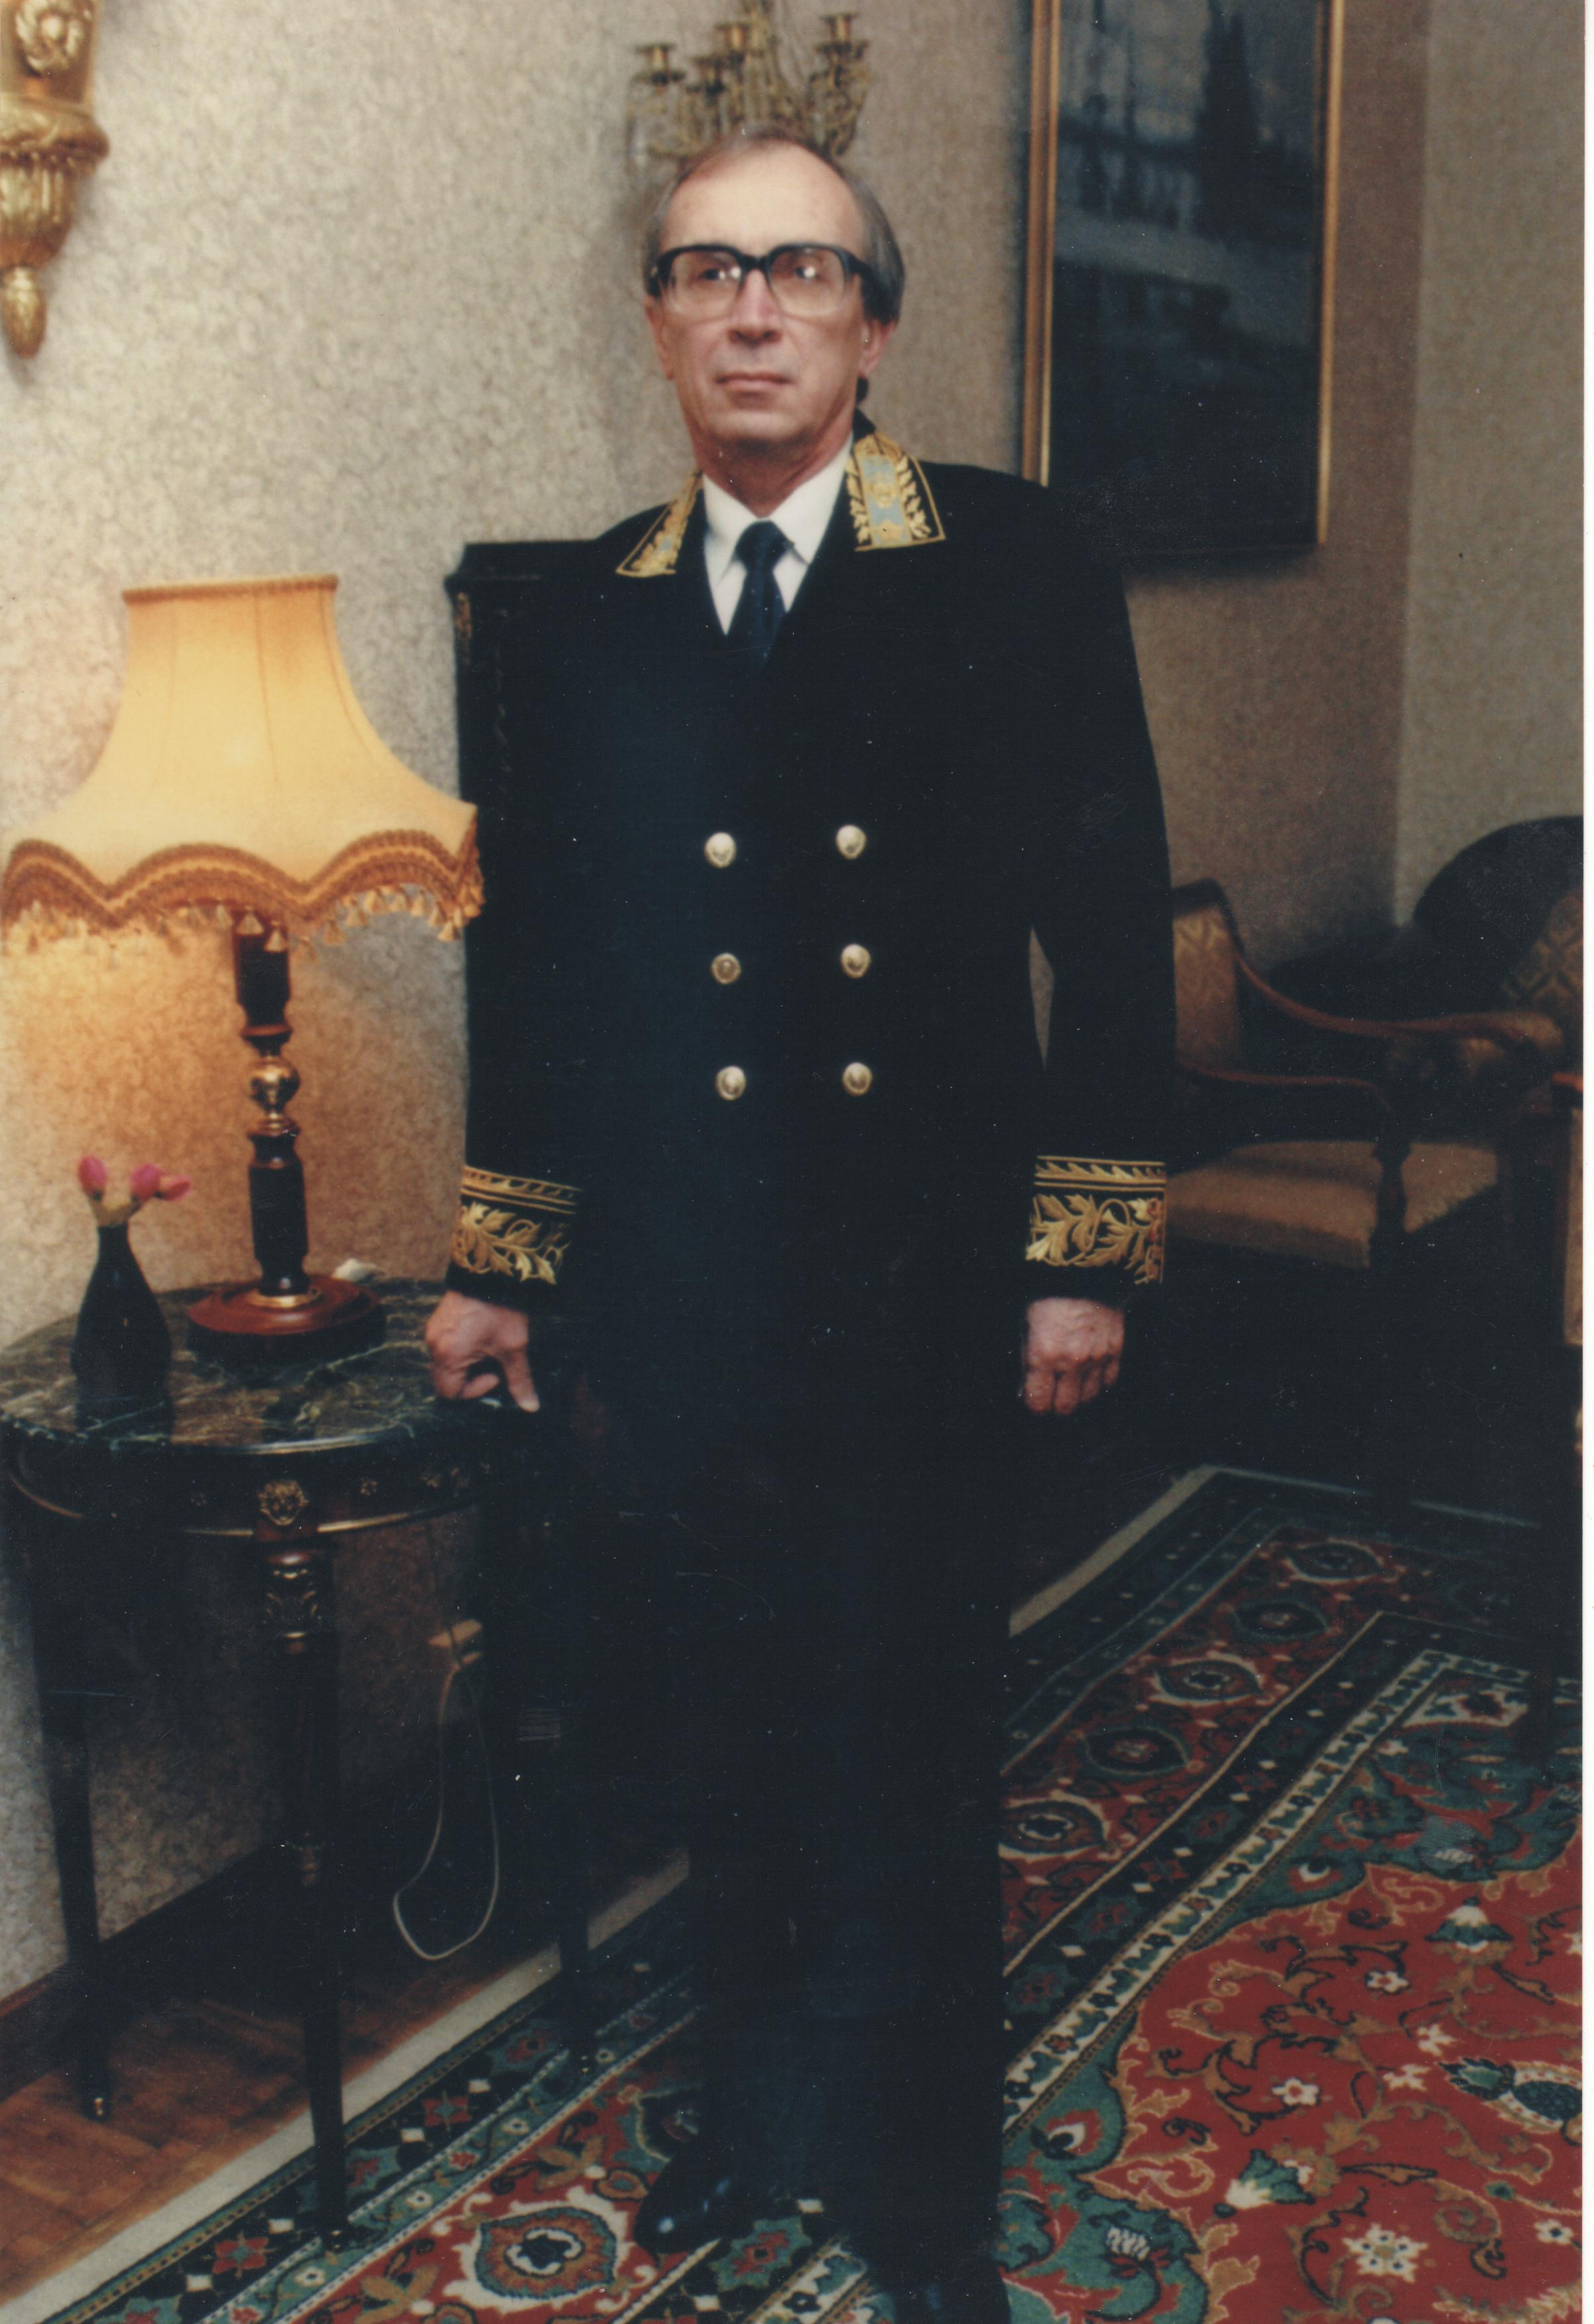
\includegraphics[height=105mm]{inc/77/1}
        \caption{О. А. Гриневский в форме Чрезвычайного и Полномочного Посла.}
\end{figure}

\begin{figure}[ht!]
    \begin{minipage}{100mm}
        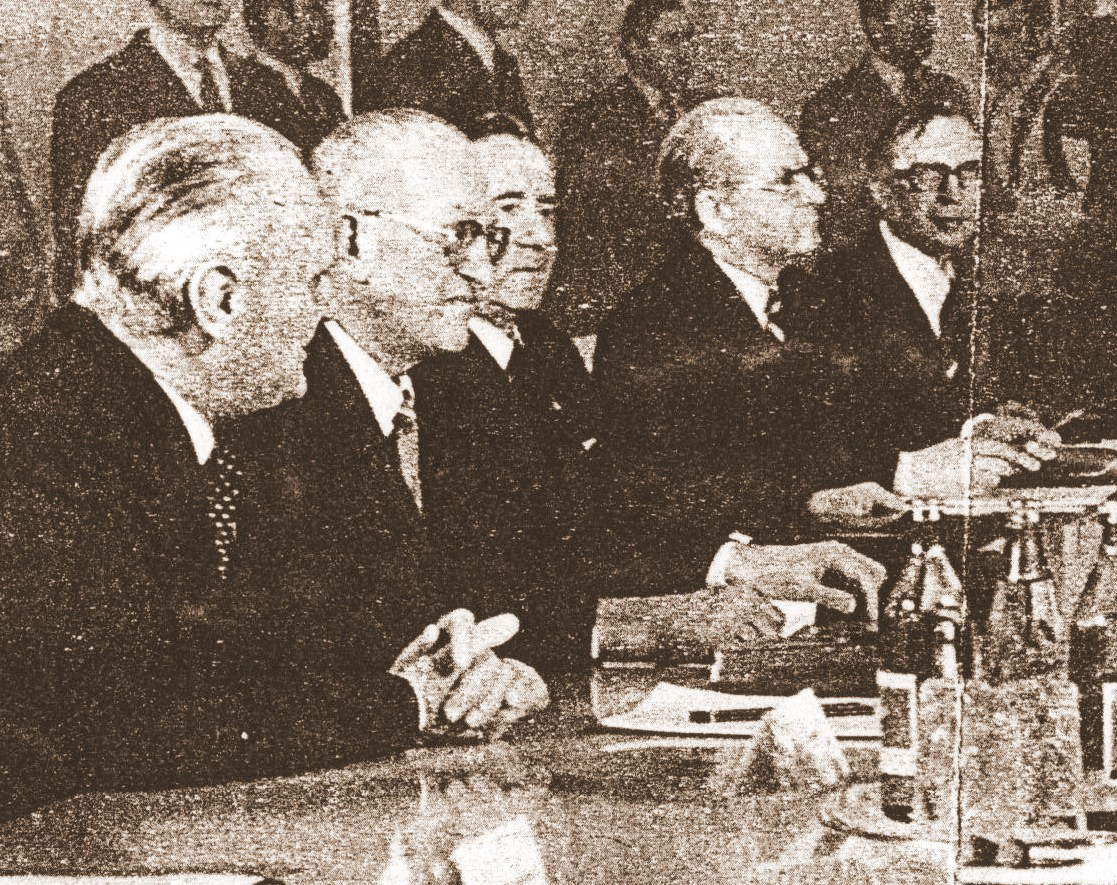
\includegraphics[width=100mm]{inc/77/2}
        \footnotesize{\textit{На международных переговорах. Первый справа~-- О. А. Гриневский.}}
     \end{minipage}
\end{figure}

\vspace{10pt}

\begin{figure}[h!]
\begin{minipage}{100mm}
    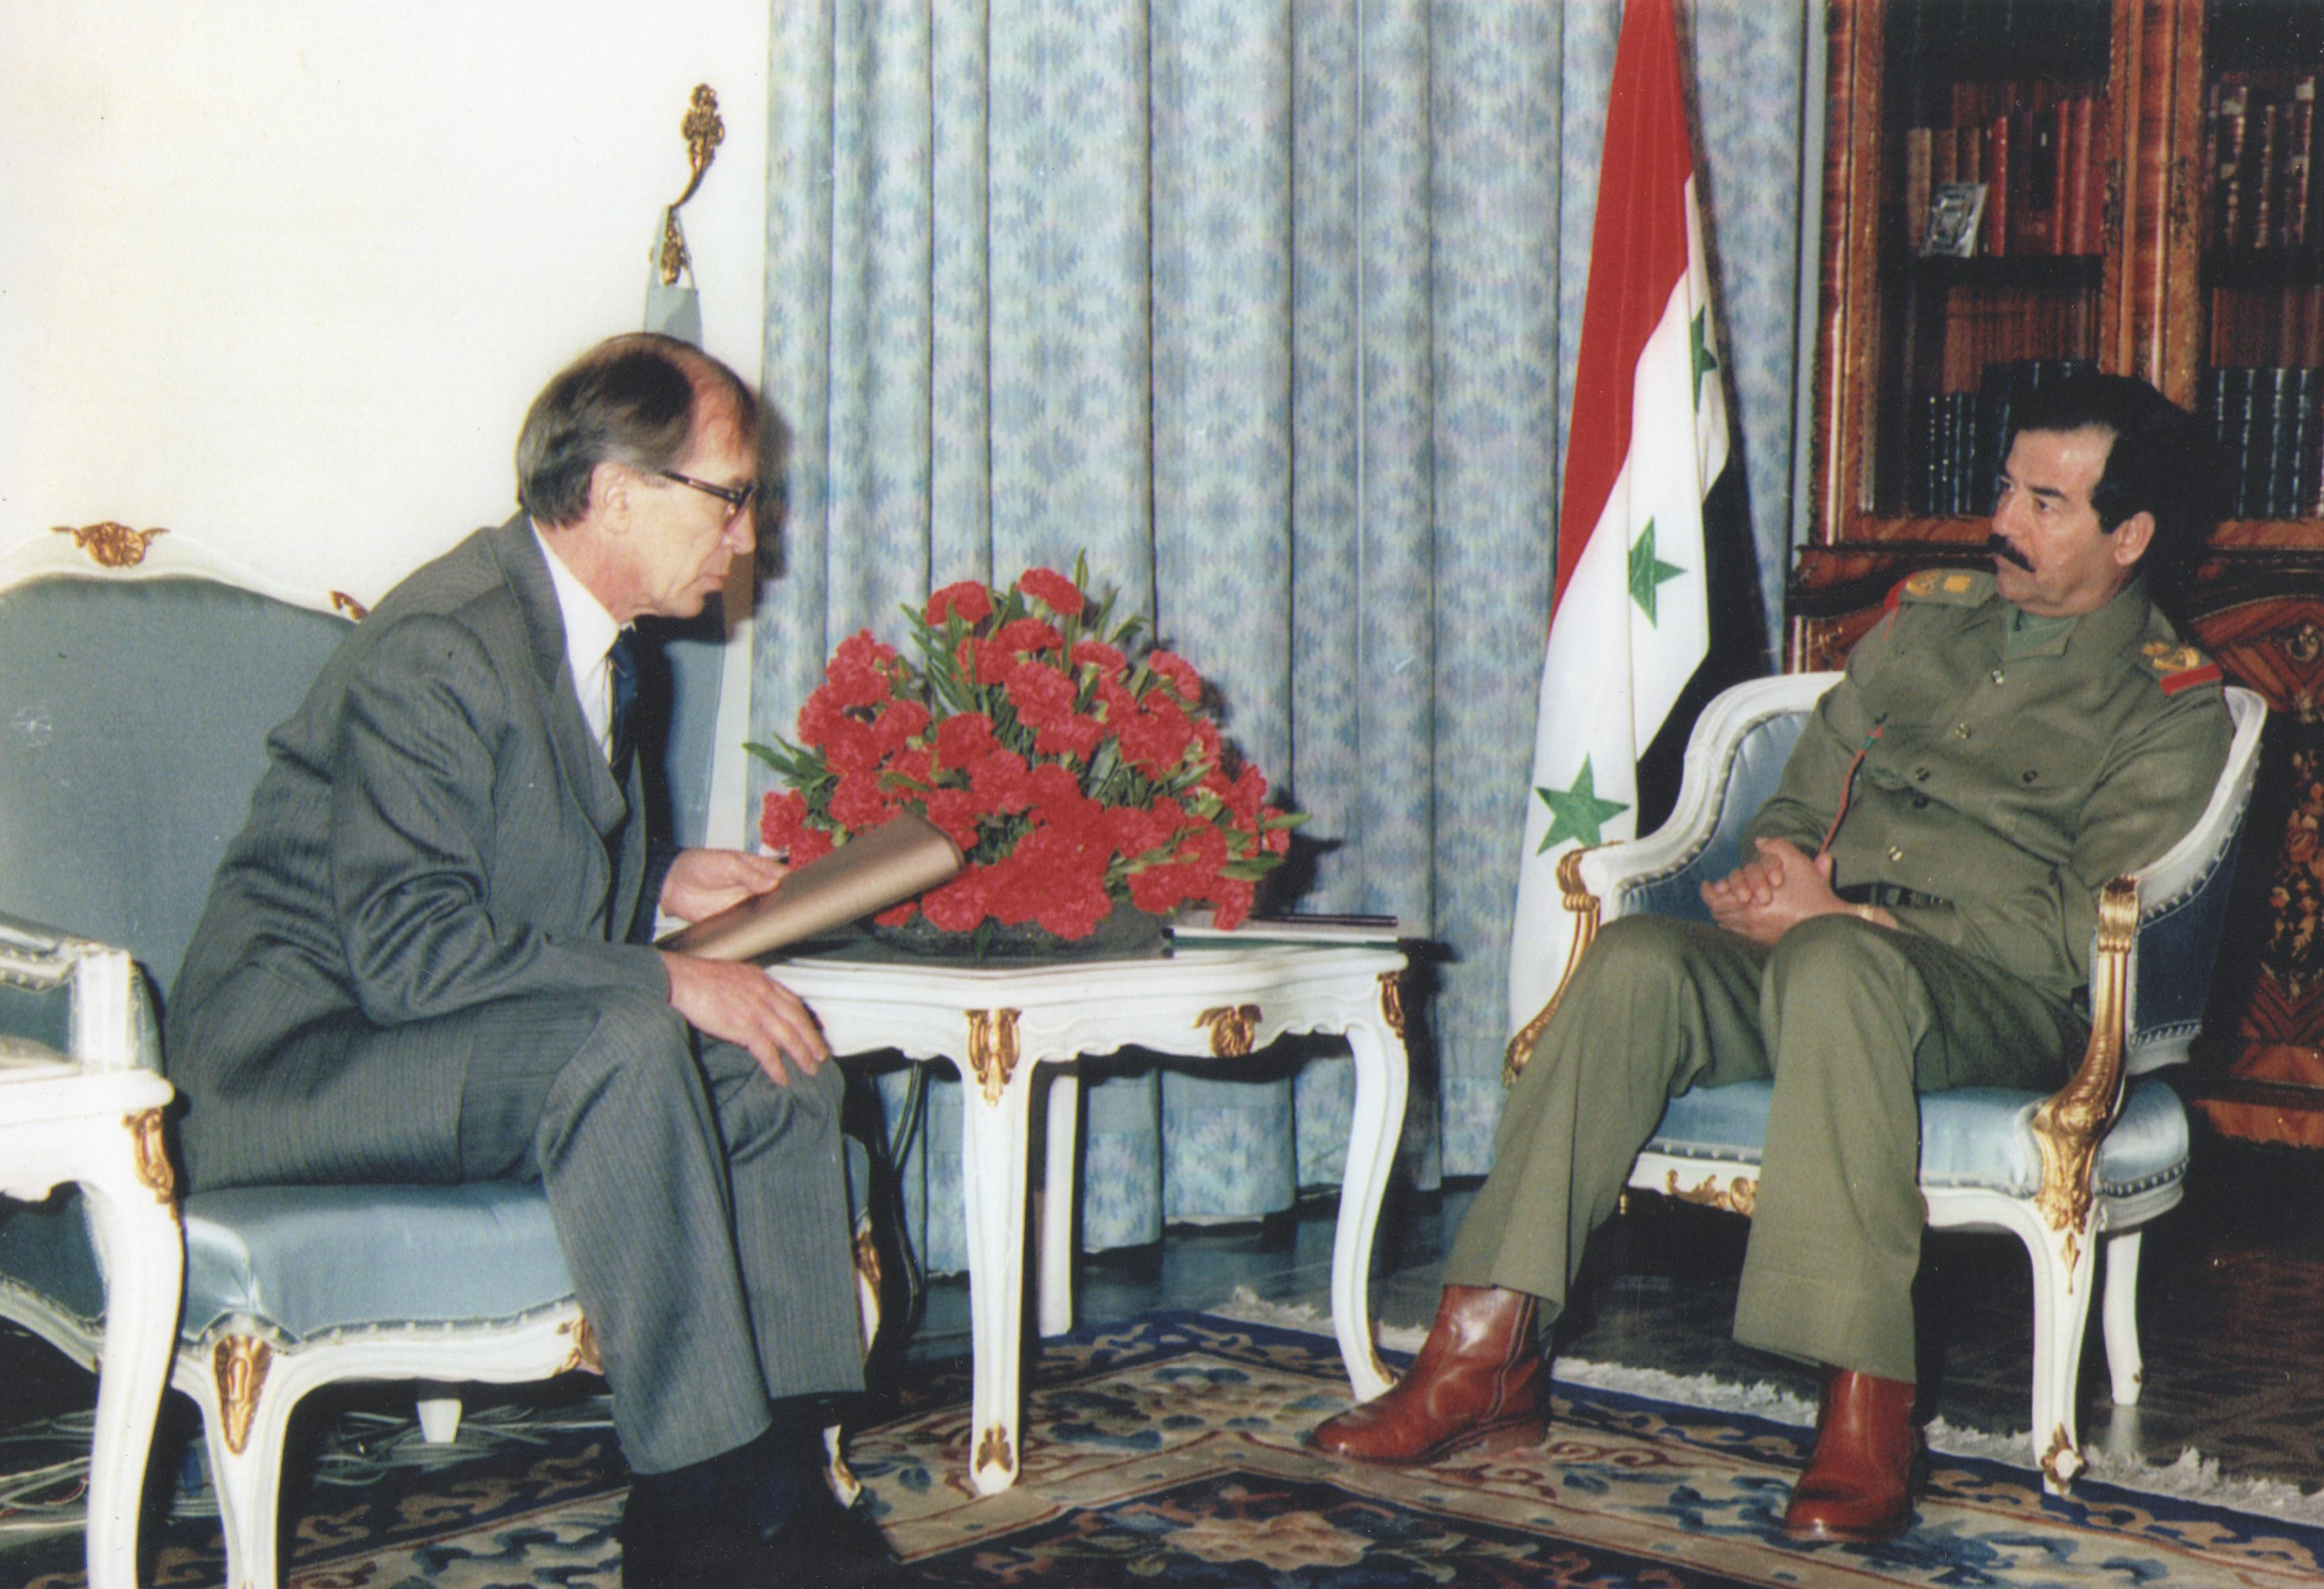
\includegraphics[width=100mm]{inc/77/3}
    \footnotesize{\textit{В духе того времени.}}
\end{minipage}
\end{figure}

